\subsection{Section 6.1 Triangulating Spaces}
\label{sec:Triangulating-Spaces}

He gave to examples first,
\begin{ex}
    A trivial example:
    \begin{figure}[H]
        \centering
        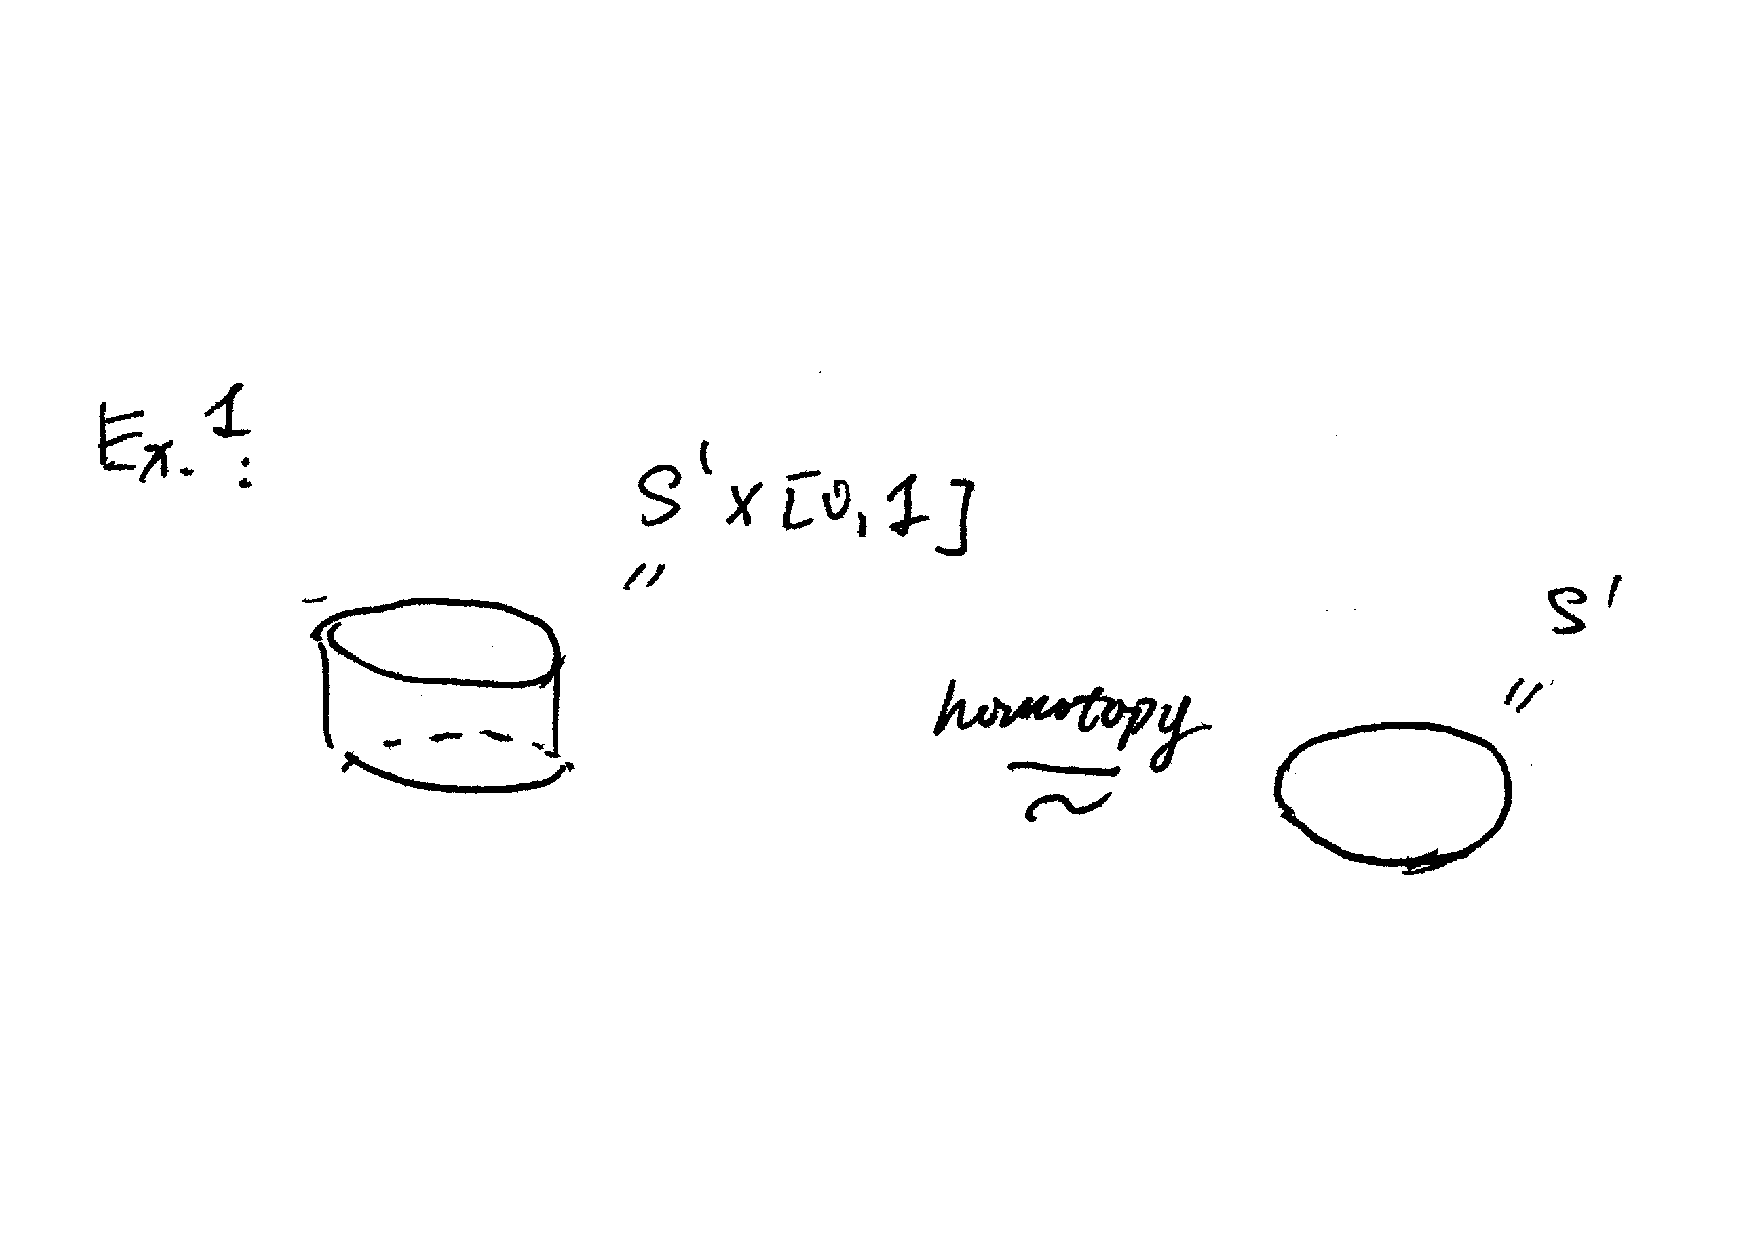
\includegraphics[width=0.6\linewidth]{pics/ch6-scanned-notes-1/ex1.pdf}
    \end{figure}
\end{ex}
\begin{ex}
    A non trivial one. That is, the M\"obius Strip also has the
    homotopy type of a ciclr $S^1$.
    \begin{figure}[H]
        \centering
        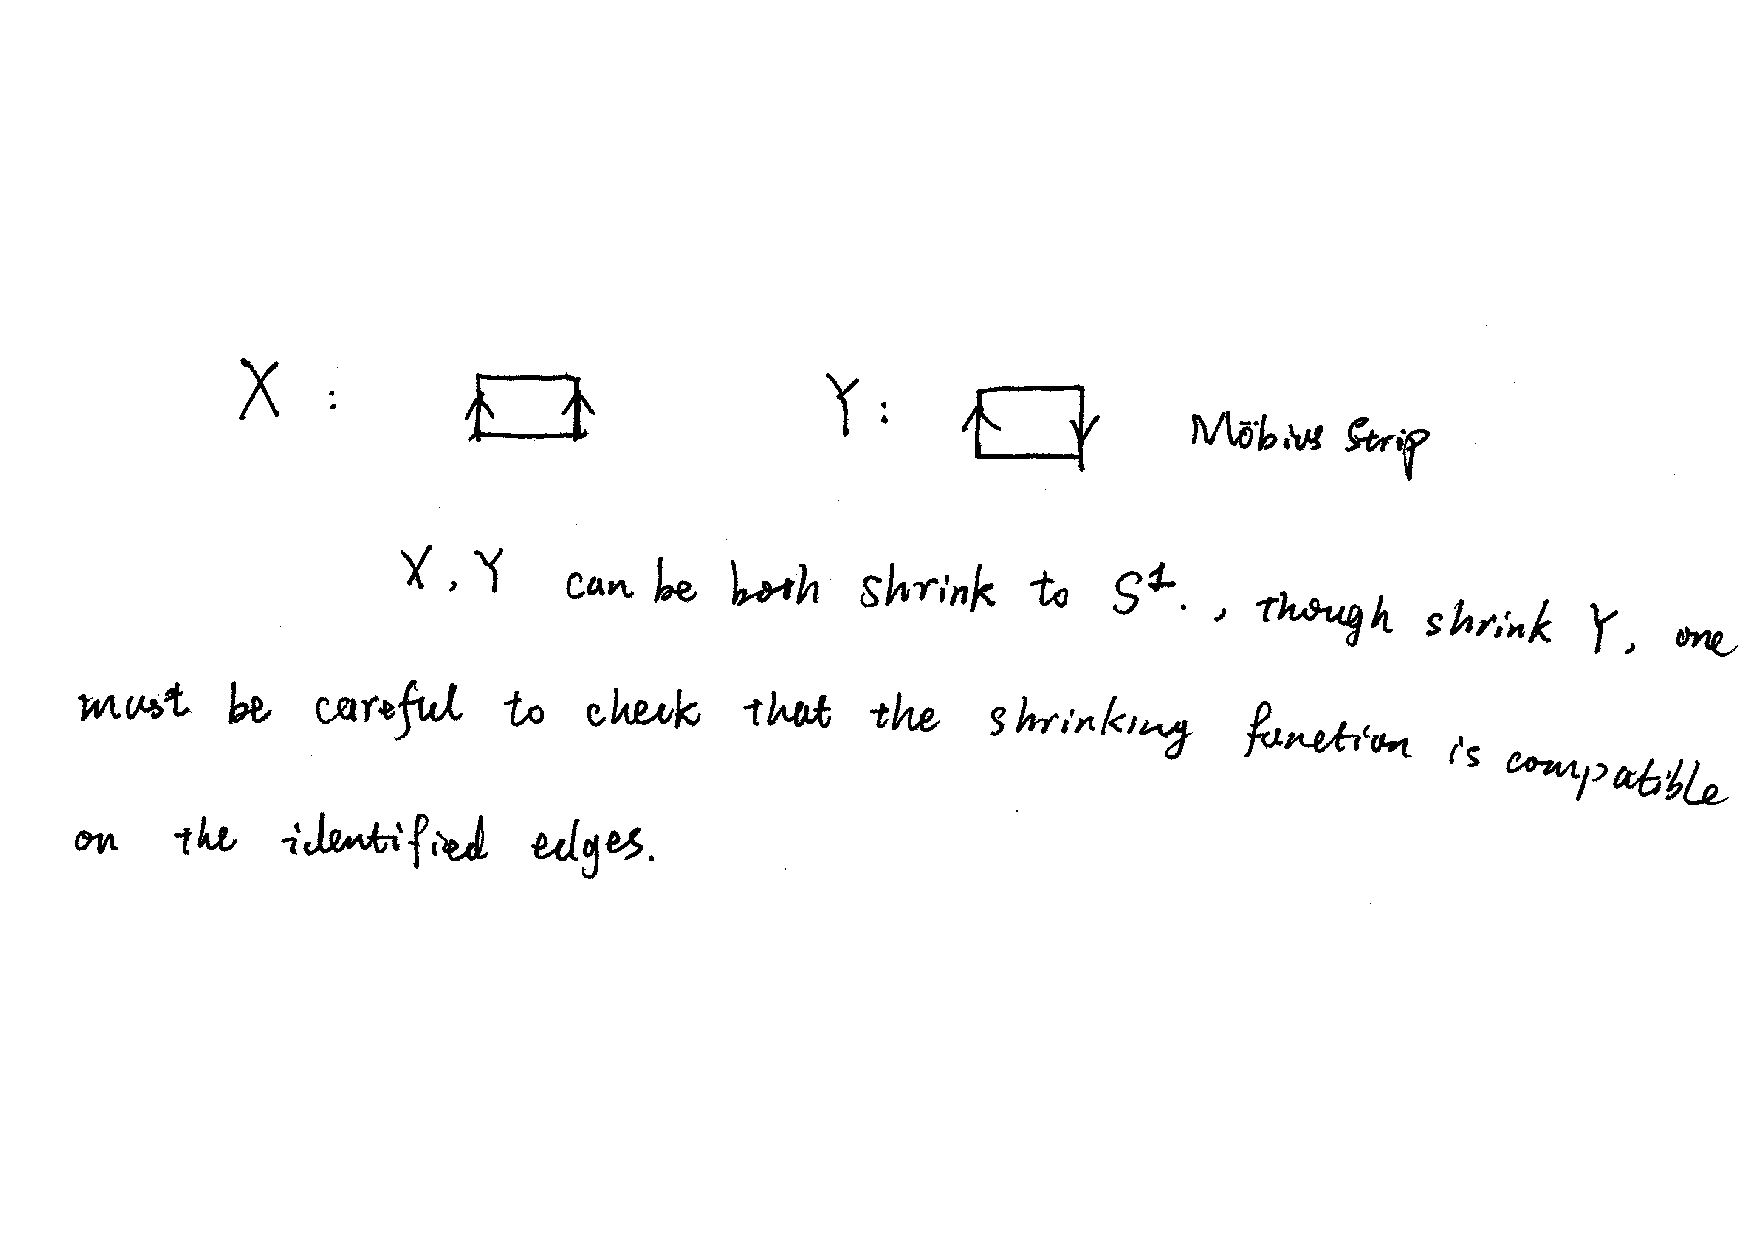
\includegraphics[width=0.8\linewidth]{pics/ch6-scanned-notes-1/ex2.pdf}
    \end{figure}
\end{ex}
But for complicated spaces, its homotopy type will not be so easy to
calculate in with simple imagination. Here we will introduce a new
technique to actually calculate the homotopy type of topological
spaces.

The technique is called Triangulation. The most visual example comes
from the computer vision technology (though I cannot find a picture by
directly Googling triangulation). The idea we wants to stress is that
the Triangulation is like use small patches of triangles to patch and
cover the surface of 3D smooth objects. Increase the overall number of
patches and make each patch get smaller. In the limit of this process
one might get to recover the original image.

\begin{defi}[Simplex of $\dim k$]
\nomenclature{Simplex of $\dim k$}{\nomrefpage.}
    The stanford simplex of $\dim k$ in $R^{k+1}$ is defined as
    follows. Let $v_i=(0,\cdots,0,1,0,\cdots 0)$, where $1$ is in $i+1$
    coordinates. That is:
    $$ v_0=(1,0,\cdots)$$
    $$ v_1=(0,1,0\cdots)$$
    $$\cdots$$
    $$ v_0=(0,\cdots,0,1)$$
    Then the simplex is the smallest convex set containing
    $\{v_0,\cdots,v_k\}$ in $\R^{k+1}$. It is also called a
    \nomen{$k$-simplex}.
\end{defi}
\begin{ex}
    \begin{figure}[H]
        \centering
        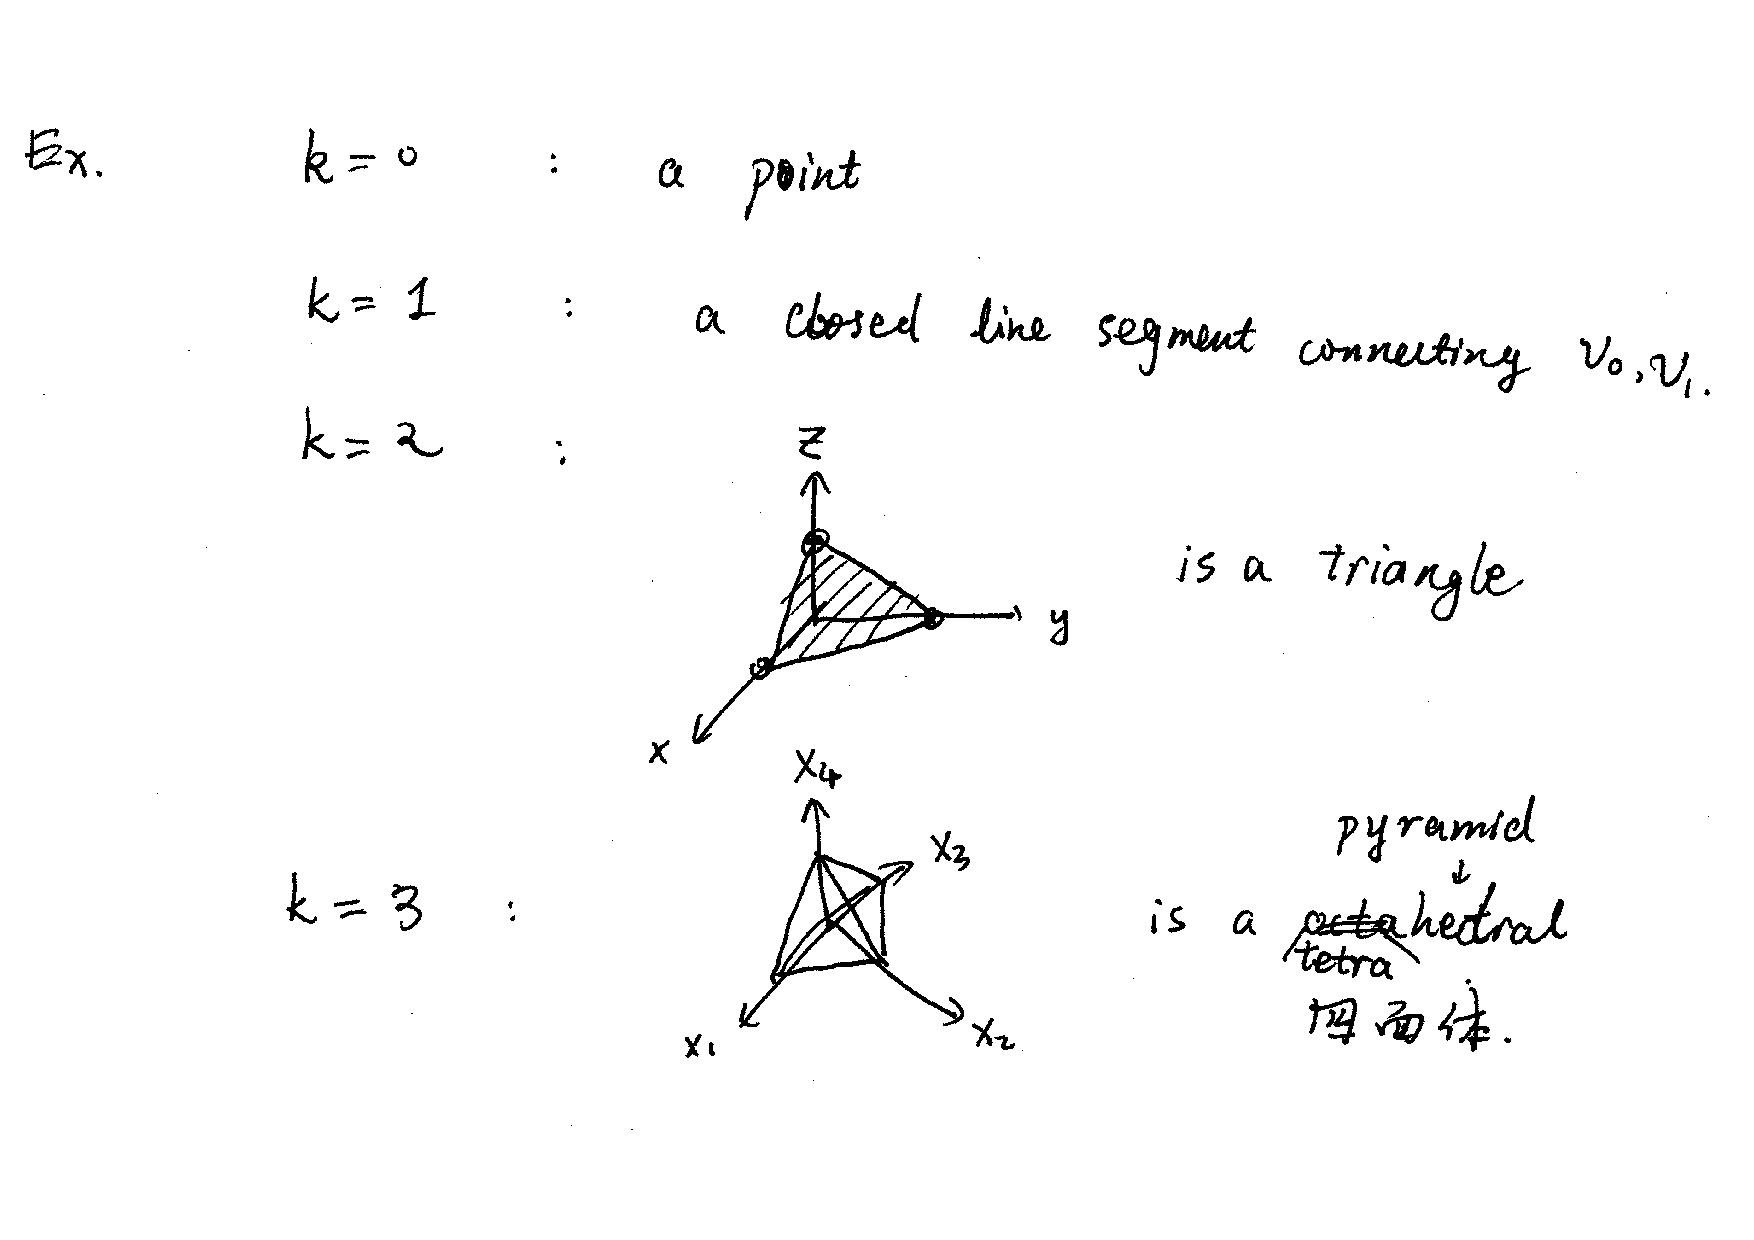
\includegraphics[width=0.8\linewidth]{pics/ch6-scanned-notes-1/ex3.pdf}
    \end{figure}
\end{ex}
\begin{fact}
    Any point in a $k$-simplex is of the form:
    \begin{equation}
        \lambda_0 v_0 + \lambda_1 v_1 + \cdots + \lambda_k v_k
    \end{equation}
    where each $\lambda_i\geq 0$, and $\sum_{i=0}^{k} \lambda_k=1$.
\end{fact}
\begin{ex}
    There is a special point in the $k$-simplex:
    \begin{equation}
        \frac{1}{k+1} \sum_{i=0}^k v_i
    \end{equation}
    When $k=2$, this is just the usual center of gravity of triangle.
\end{ex}

We want to study those space which is the union of a finite collection
of simplexes which fit together nicely in some Euclidean space. These
are called "triangulable spaces". More specifically:
\begin{defi}[faces]
\nomenclature{faces}{\nomrefpage.}
    If $A$ and $B$ are simplexes, and if the vertices of $B$ form a
    subset of vertices of $A$. Then $B$ is called a face of $A$,
    written as \nomen{$B<A$}.
\end{defi}
\begin{defi}[Simplicial Complex]
\nomenclature{Simplicial Complex}{\nomrefpage.}
    A \textbf{finite} collection of simplexes in some Euclidean space
    in $\R^n$ is called a simplicial complex, if
    \begin{enumerate}
        \item whenever a simplex lies in this collection, then so does
            its faces
        \item whenever two simplexes in this collection intersect,
            their intersection is a common face of these two
            simplexes.
    \end{enumerate}
\end{defi}
\begin{ex}
    % ex 4
\end{ex}
\begin{defi}[Topology on simplicial complex]
\nomenclature{Topology on simplicial complex}{\nomrefpage.}
    The topology on a simplicial complex is given by the subspace
    topology of Euclidean space. Let $K$ be a simplicial complex, we
    denote \nomen{$|K|$} as the topology of $K$. This $|K|$ is called
    a \nomen{polyhedron}.
\end{defi}

\begin{defi}[Triangulation and Triangulable]
\nomenclature{Triangulation and Triangulable}{\nomrefpage.}
    A triangulation on a topological space $X$ consists of a
    simplicial complex $K$, and a homeomorphism $h$:
    $$ h:|K|\to X$$
    A space is called triangulable if such simplicial complex $|K|$
    and homeomorphism $h$ exists.
\end{defi}
\begin{fact}
    If $X$ is triangulable, then $X$ is compact and can be made into a
    metric space. (Notice that the simplicial complex is a finite
    collection.)
\end{fact}
\begin{remark}
    Trigulation is in general not unique. For example:
    \begin{figure}[H]
        \centering
        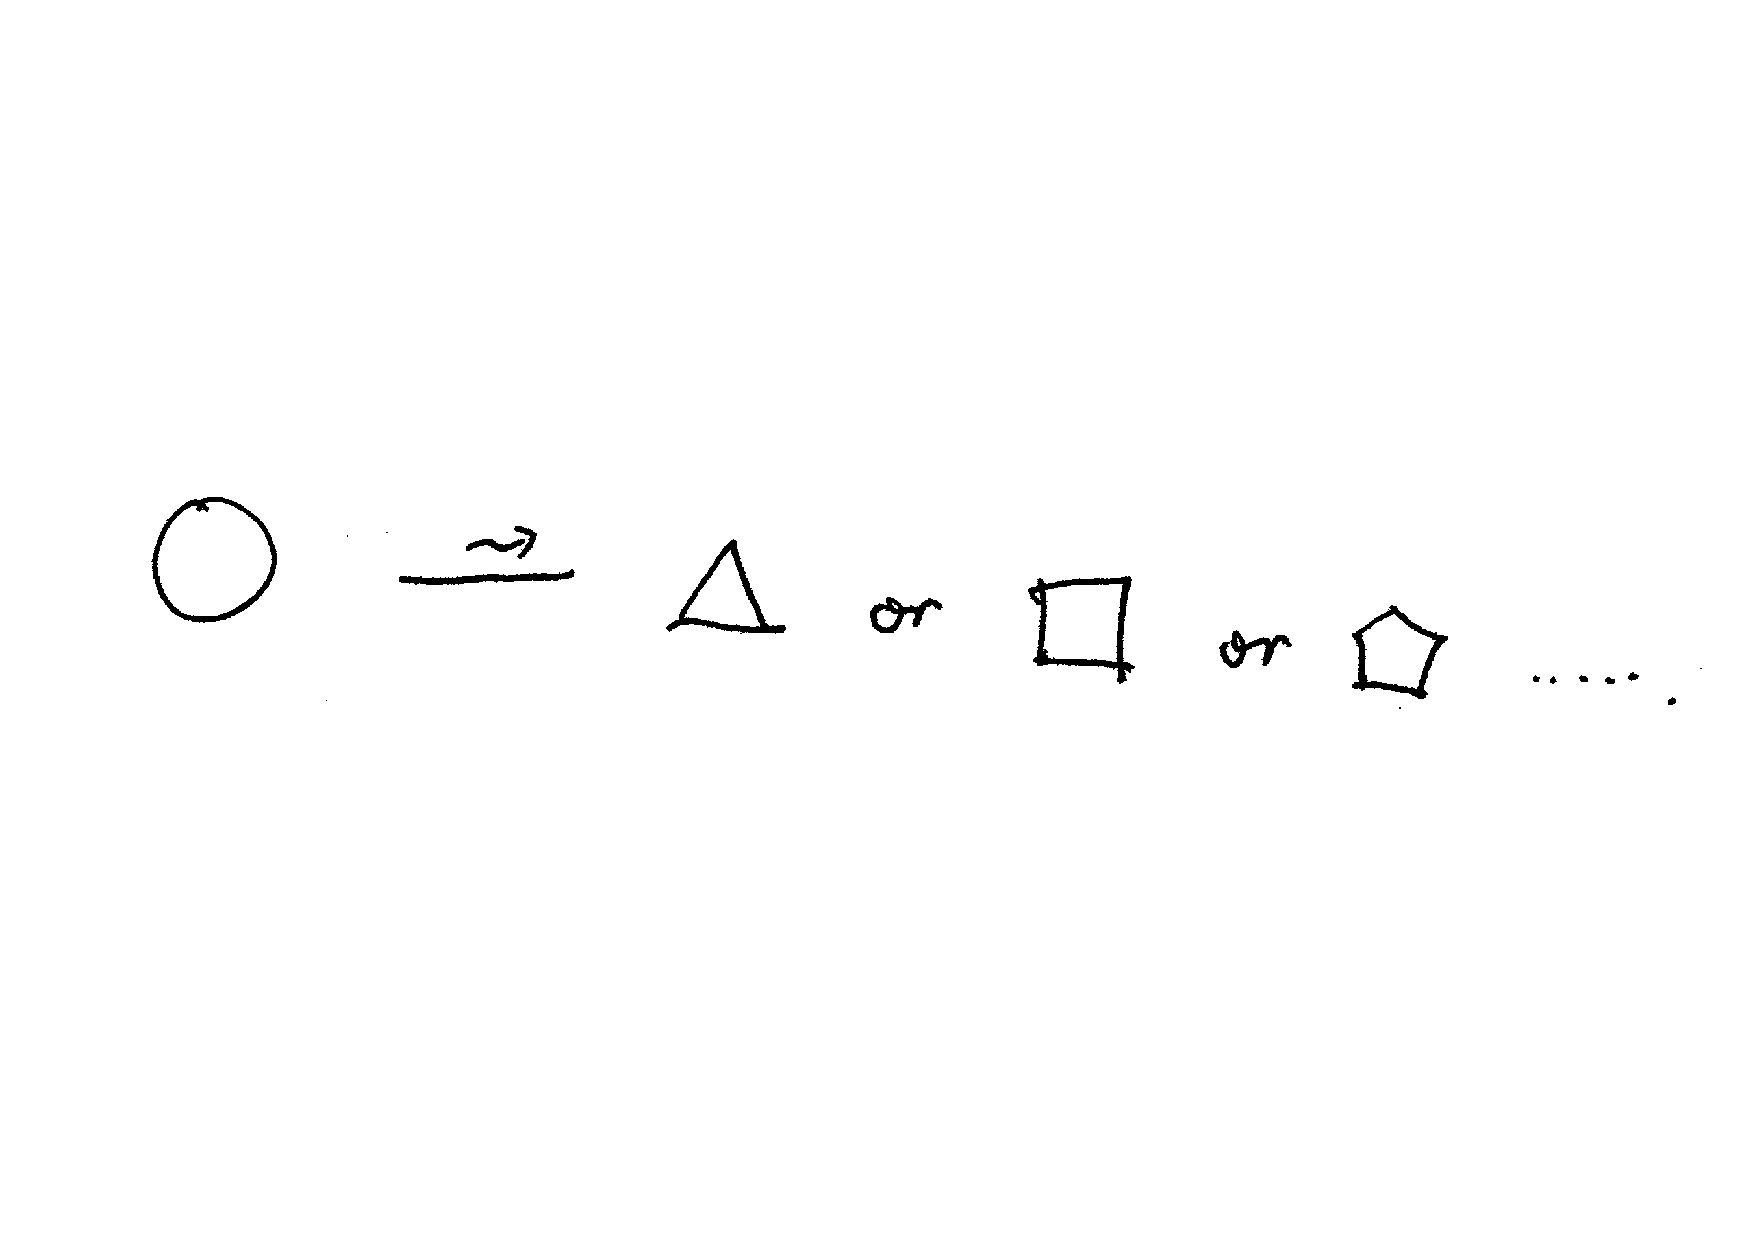
\includegraphics[width=0.6\linewidth]{pics/ch6-scanned-notes-1/rmk2}
    \end{figure}
\end{remark}
\begin{ex}
    \label{ex:triangu-torus}
    Here is a triangulation on the torus:
    \begin{figure}[H]
        \centering
        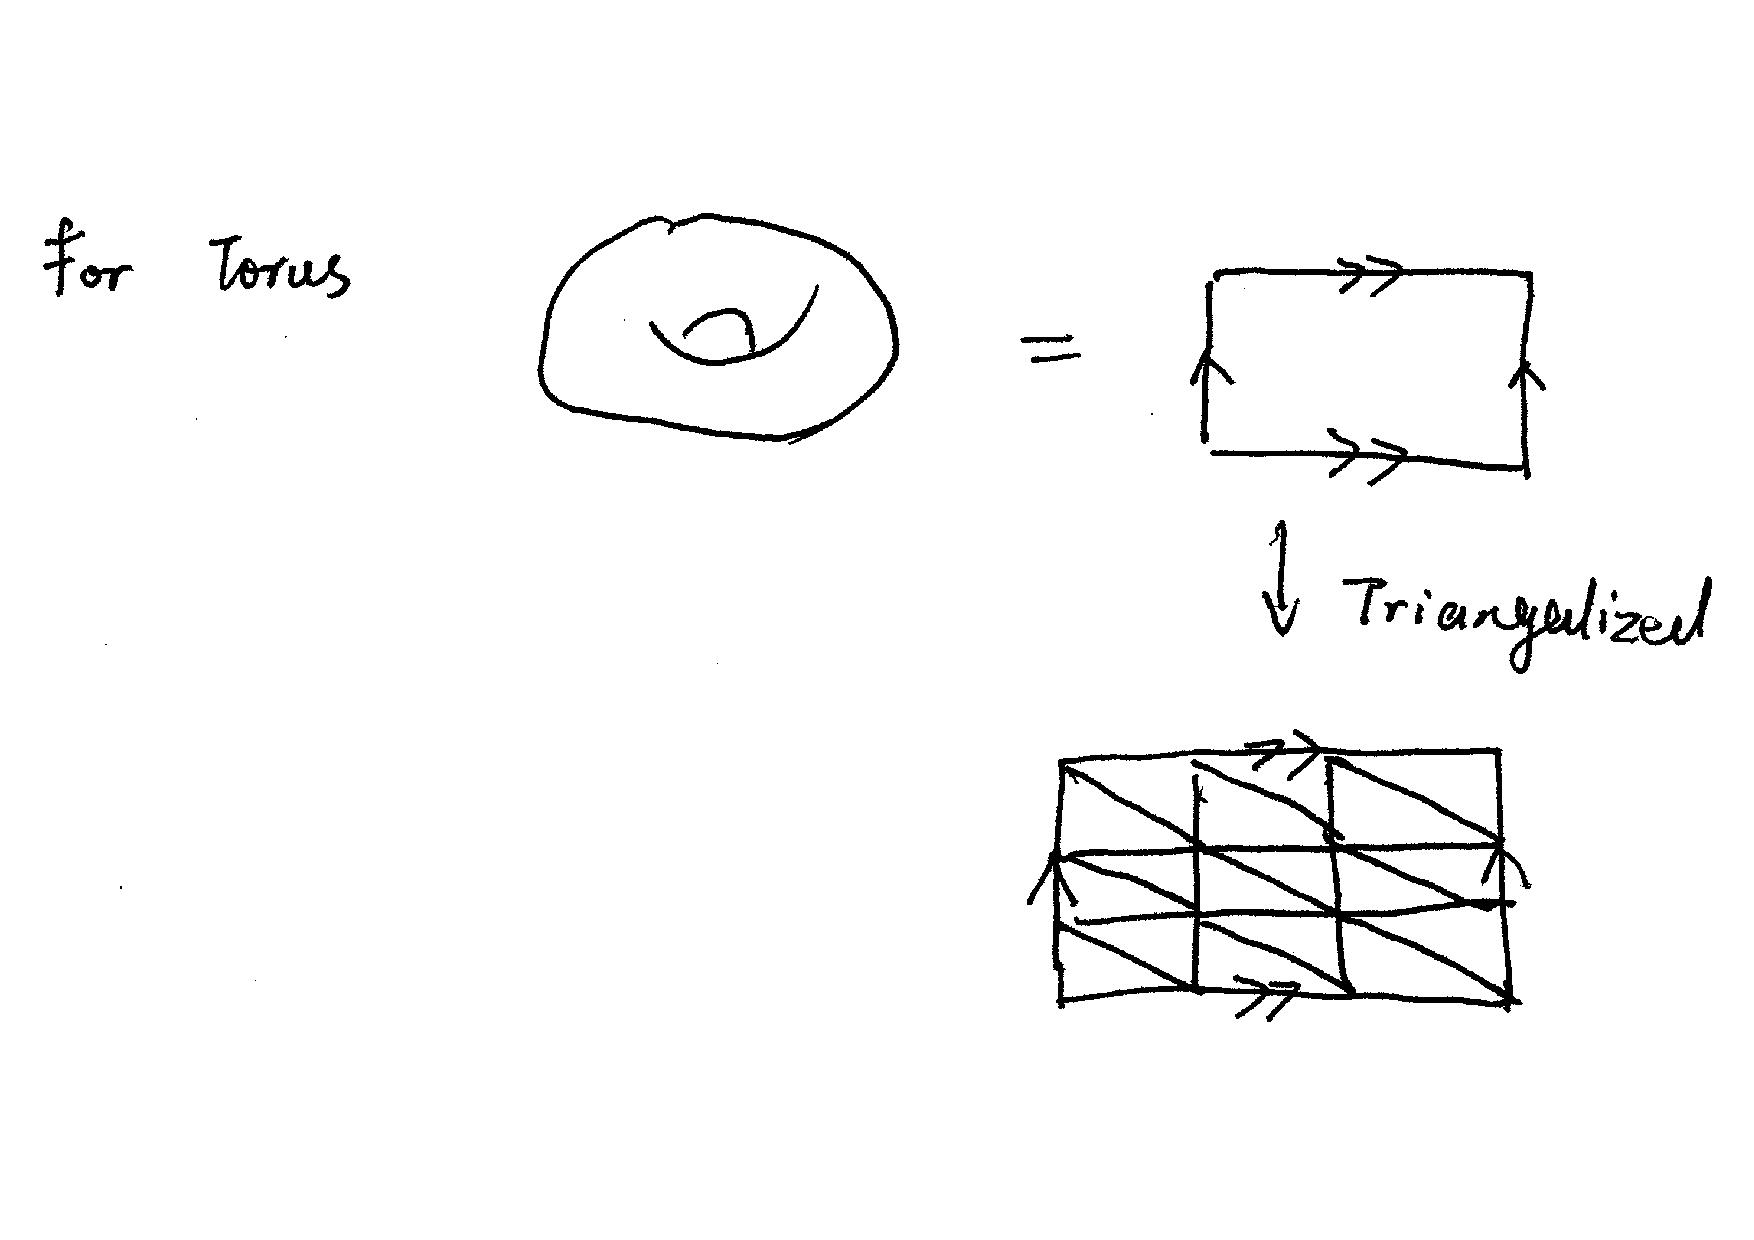
\includegraphics[width=0.6\linewidth]{pics/ch6-scanned-notes-1/p5.pdf}
    \end{figure}
    Notice that the following diagram is not a triangulation of torus:
    \begin{figure}[H]
        \centering
        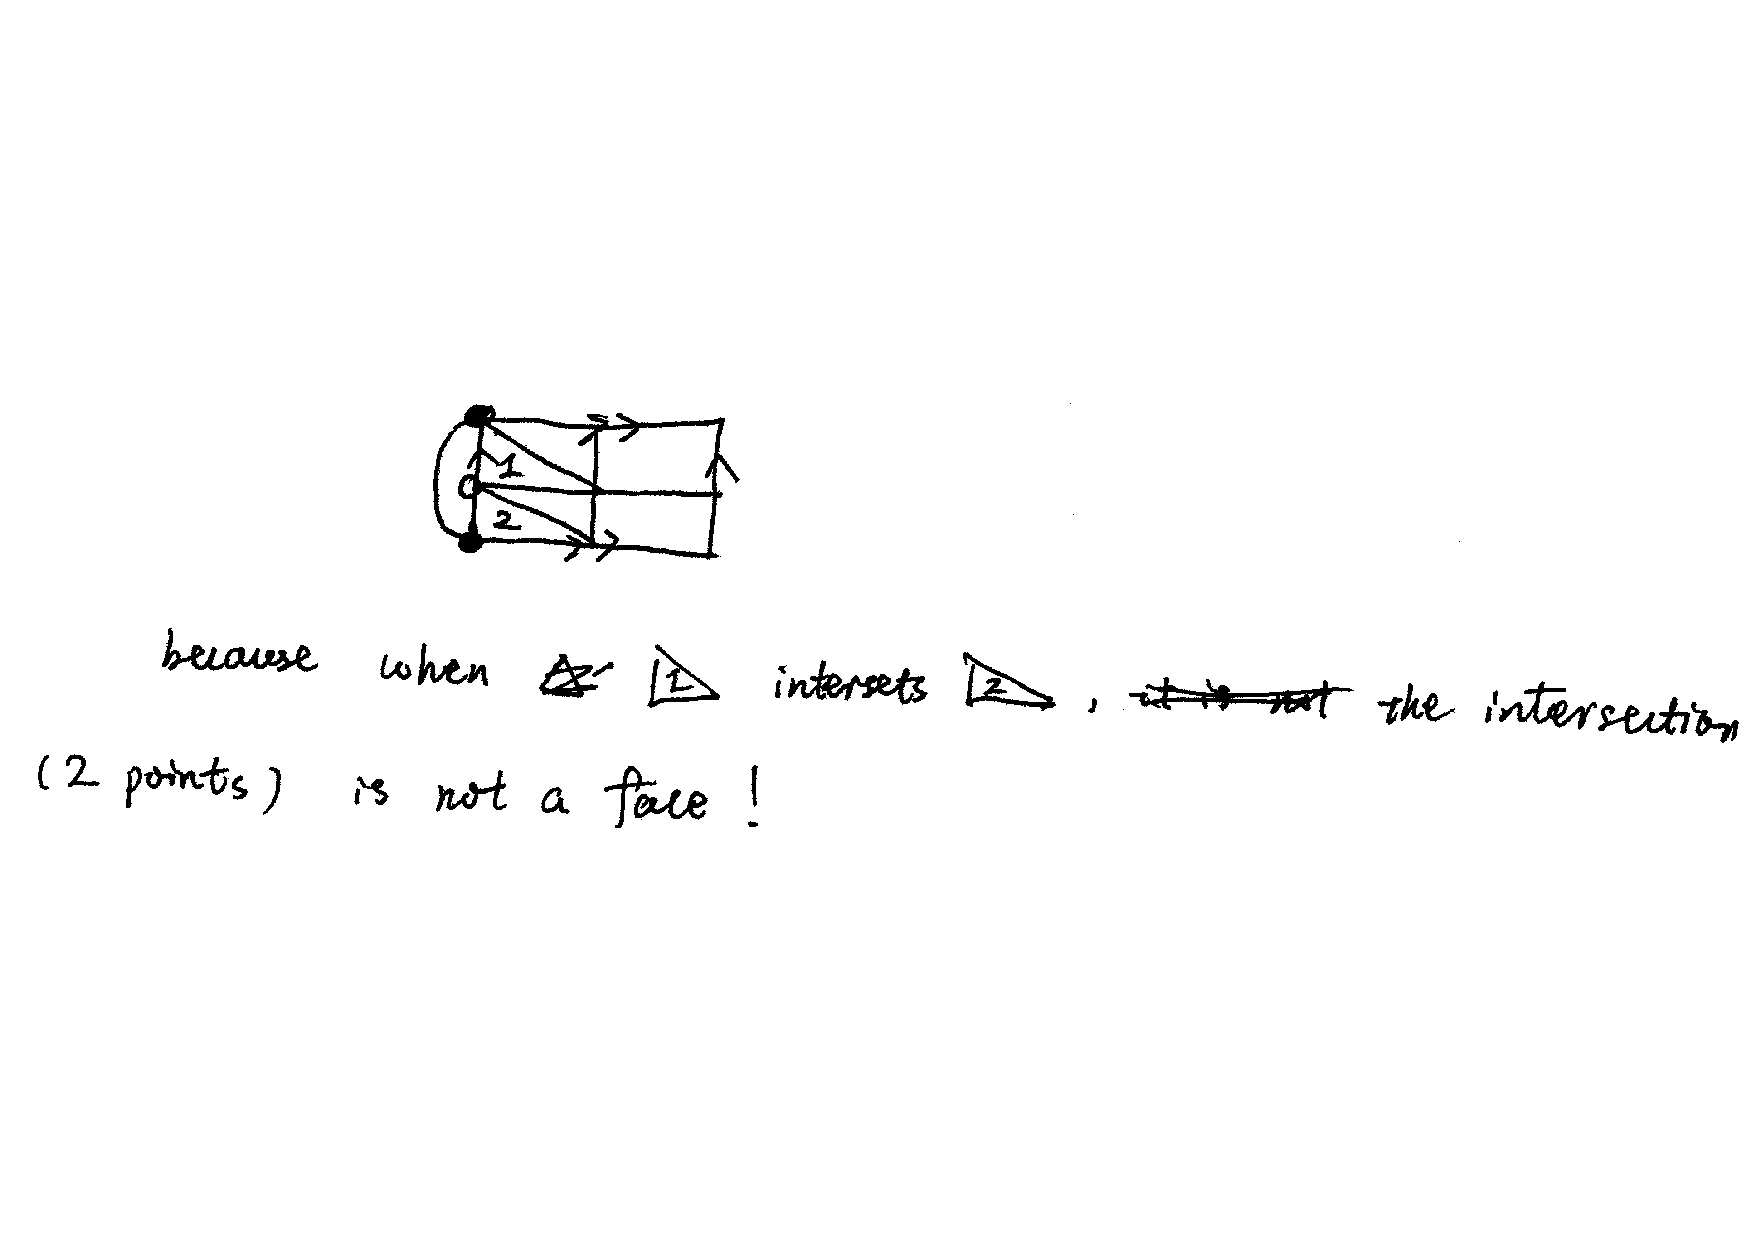
\includegraphics[width=0.8\linewidth]{pics/ch6-scanned-notes-1/p52.pdf}
    \end{figure}
\end{ex}
\begin{lemma}
    Let $K$ be a simplicial complex in $\R^{n}$, then
    \begin{enumerate}
        \item $|K|$ is compact.
        \item Each point of $|K|$ lies in the interior of exactly one
            simplex of $K$.
        \item If we take the simplexes of $K$ seperately, and give
            their union the identification topology, we obtain $|K|$.
            Thus we have two equivalent ways to view the topology on
            $K$.
        \item If $|K|$ is connected, then $|K|$ is also
            path-connected.
    \end{enumerate}
\end{lemma}
\begin{proof}
\begin{enumerate}
    \item Obviously.
    \item Since $K$ is connected by simplexes, a point $p$ must
        obviously be contained in some simplex. Also, since on each
        simplex $p$ must be on the interior of it, or interior of its
        components. We only need to prove that the containing simplex
        is unique. Suppose $p$ is the interior of simplexes $A$ and
        $B$. Notice that their intersection must be their faces. The
        only face of $A$ or $B$ containing interior points is $A$ or
        $B$ itself. Hence $A=B$.
    \item By definition of identification topology, we can see that in
        the identified space, a subset $C\subset |K|$, $C$ is closed
        $\Leftrightarrow$ $C\cap |A|$ is closed in $|A|$ for all
        simplexes $A\in K$. The rest of the proof is obvious.
    \item We need only to show that $|K|$ is locally path-connected.
        But any point $p\in K$, $p\in$ interior of some $A$ where
        $A\in K$. That is, we can find a neighbourhood $U$ of $p$, and
        $U$ is contained in $A$ ($U\subset A$). (More specifically, we
        can find $\varepsilon$ such that 
        $B_{\varepsilon}(p)\cup |K| = B_\varepsilon(p)\cup |A|$)
        But a simplex $A$ is obviously locally path-connected. Hence
        $U$ (or $B_\varepsilon(p)$) is path connected, hence $|K|$ is
        path-connected.
\end{enumerate}
\end{proof}

\subsection{Section 6.2 Barycentric Division}
\label{sec:Barycentric-Division}
Now we begin to make the triangulation more and more detailed. We
start from a simplicial complex $K$ and constructing a new simplicial
complex $K_1$, such that
\begin{enumerate}
    \item $|K|=|K_1|$, homeomorphically.
    \item diameter $|K_1|<$ diameter $|K|$.
\end{enumerate}
The general construction method is called Barycentric division,
visualized as:
\begin{figure}[H]
    \centering
    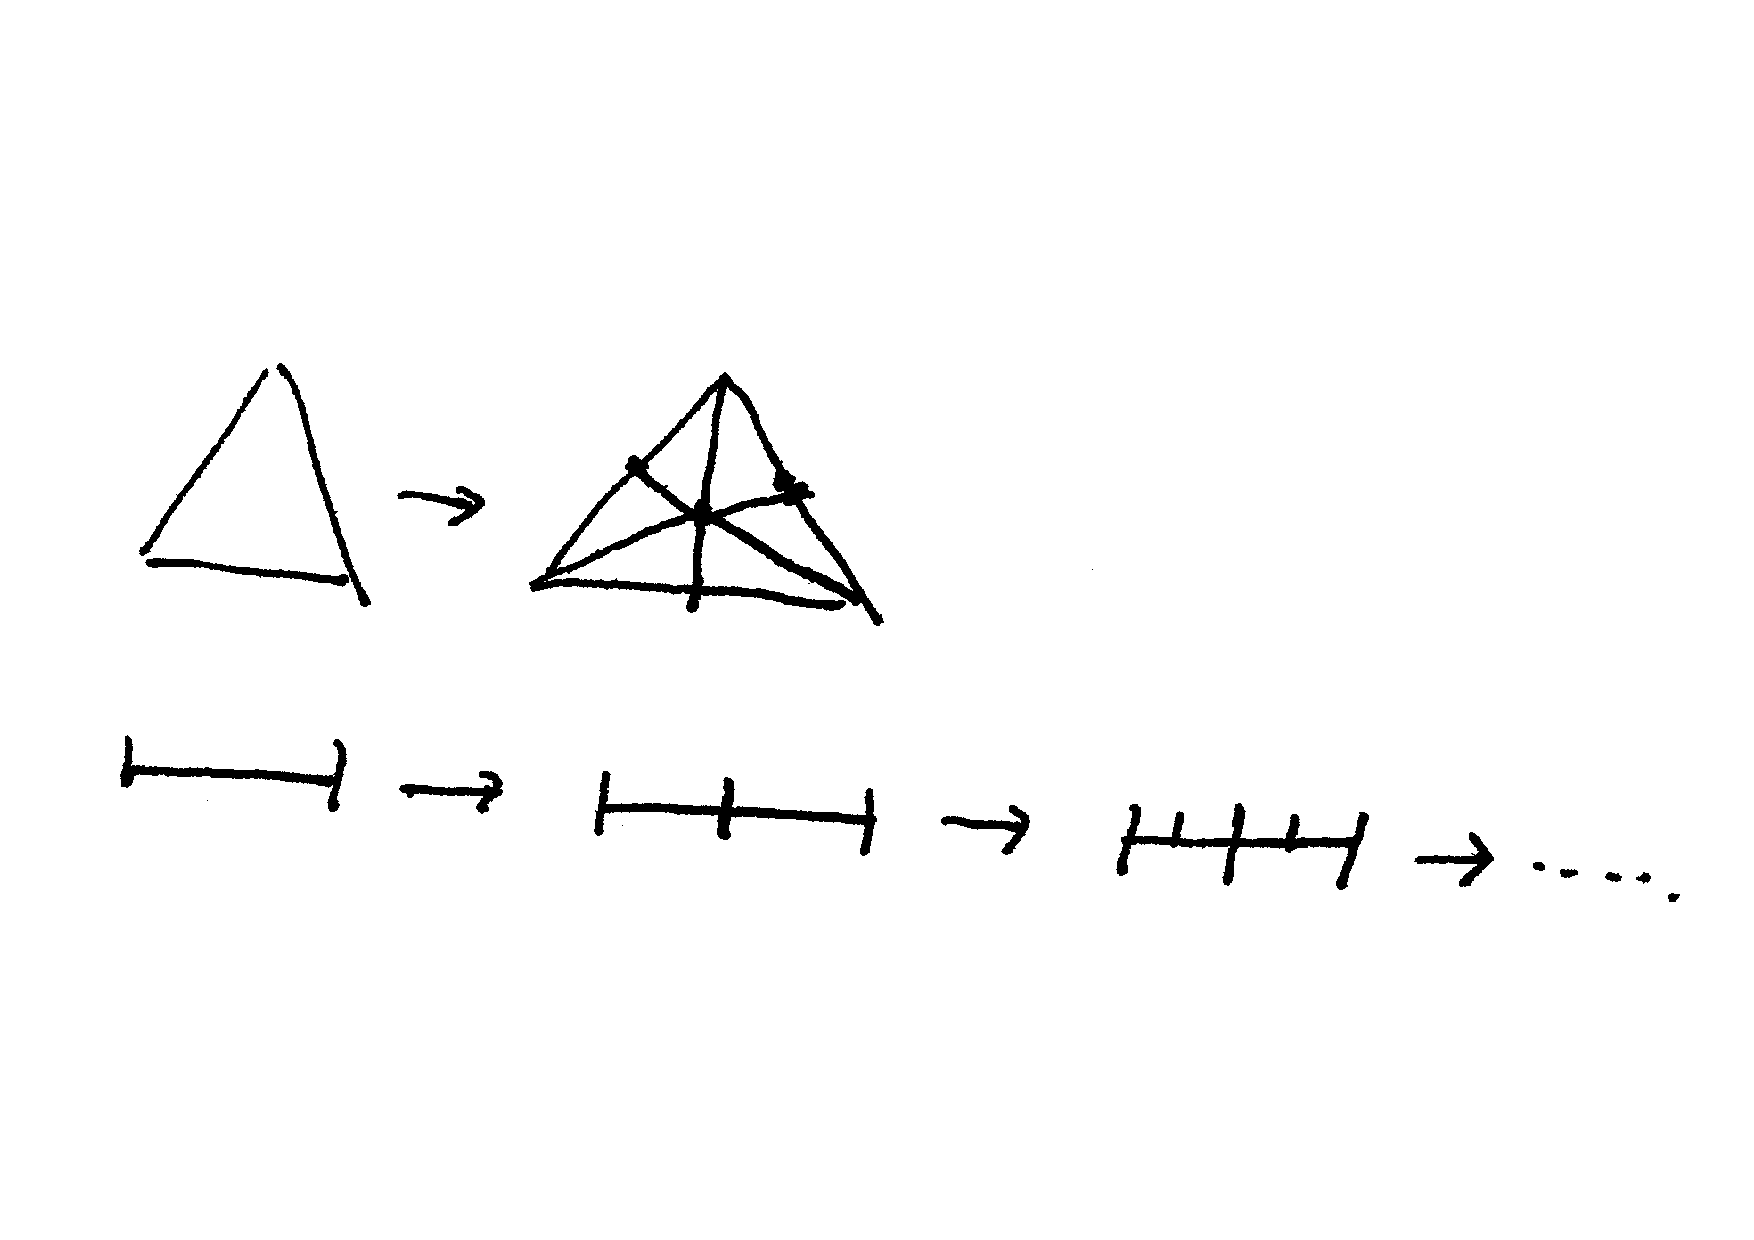
\includegraphics[width=0.6\linewidth]{pics/ch6-scanned-notes-1/8.pdf}
\end{figure}
We first define a concept
\begin{defi}[$\hat{A}$ Bary center]
\nomenclature{$\hat{A}$ Bary center}{\nomrefpage.}
Let $A$ be a simplex, then the bery center of $A$, denoted $\hat{A}$,
is the point:
\begin{equation}
    \hat{A}:= \frac{1}{k+1}(v_0+\cdots+v_k)
\end{equation}
\end{defi}
Then, the general process is:
The new space $K_1$ is such that
\begin{enumerate}
    \item The vertices of $K_1$ are bary centers of \textbf{ALL}
        simplexes of $K$. Note the the bary center of a $0$-simplex
        is just itself. So in general, $K_1$ has more vertices of
        $K$.
    \item A collection $\hat{A}_0,\cdots,\hat{A}_k$ of such bary
        centers will form a vertex of a $k$-simplex in $K_1$ if and
        only if there is a permutation $\sigma$ of $\{0,1,\cdots,k\}$
        such that
        \begin{equation}
            A_{\sigma{0}}< A_{\sigma{1}} < \cdots < A_{\sigma{k}}
        \end{equation}
\end{enumerate}
\begin{remark}
    The second point above tries to do the following
    \begin{figure}[H]
        \centering
        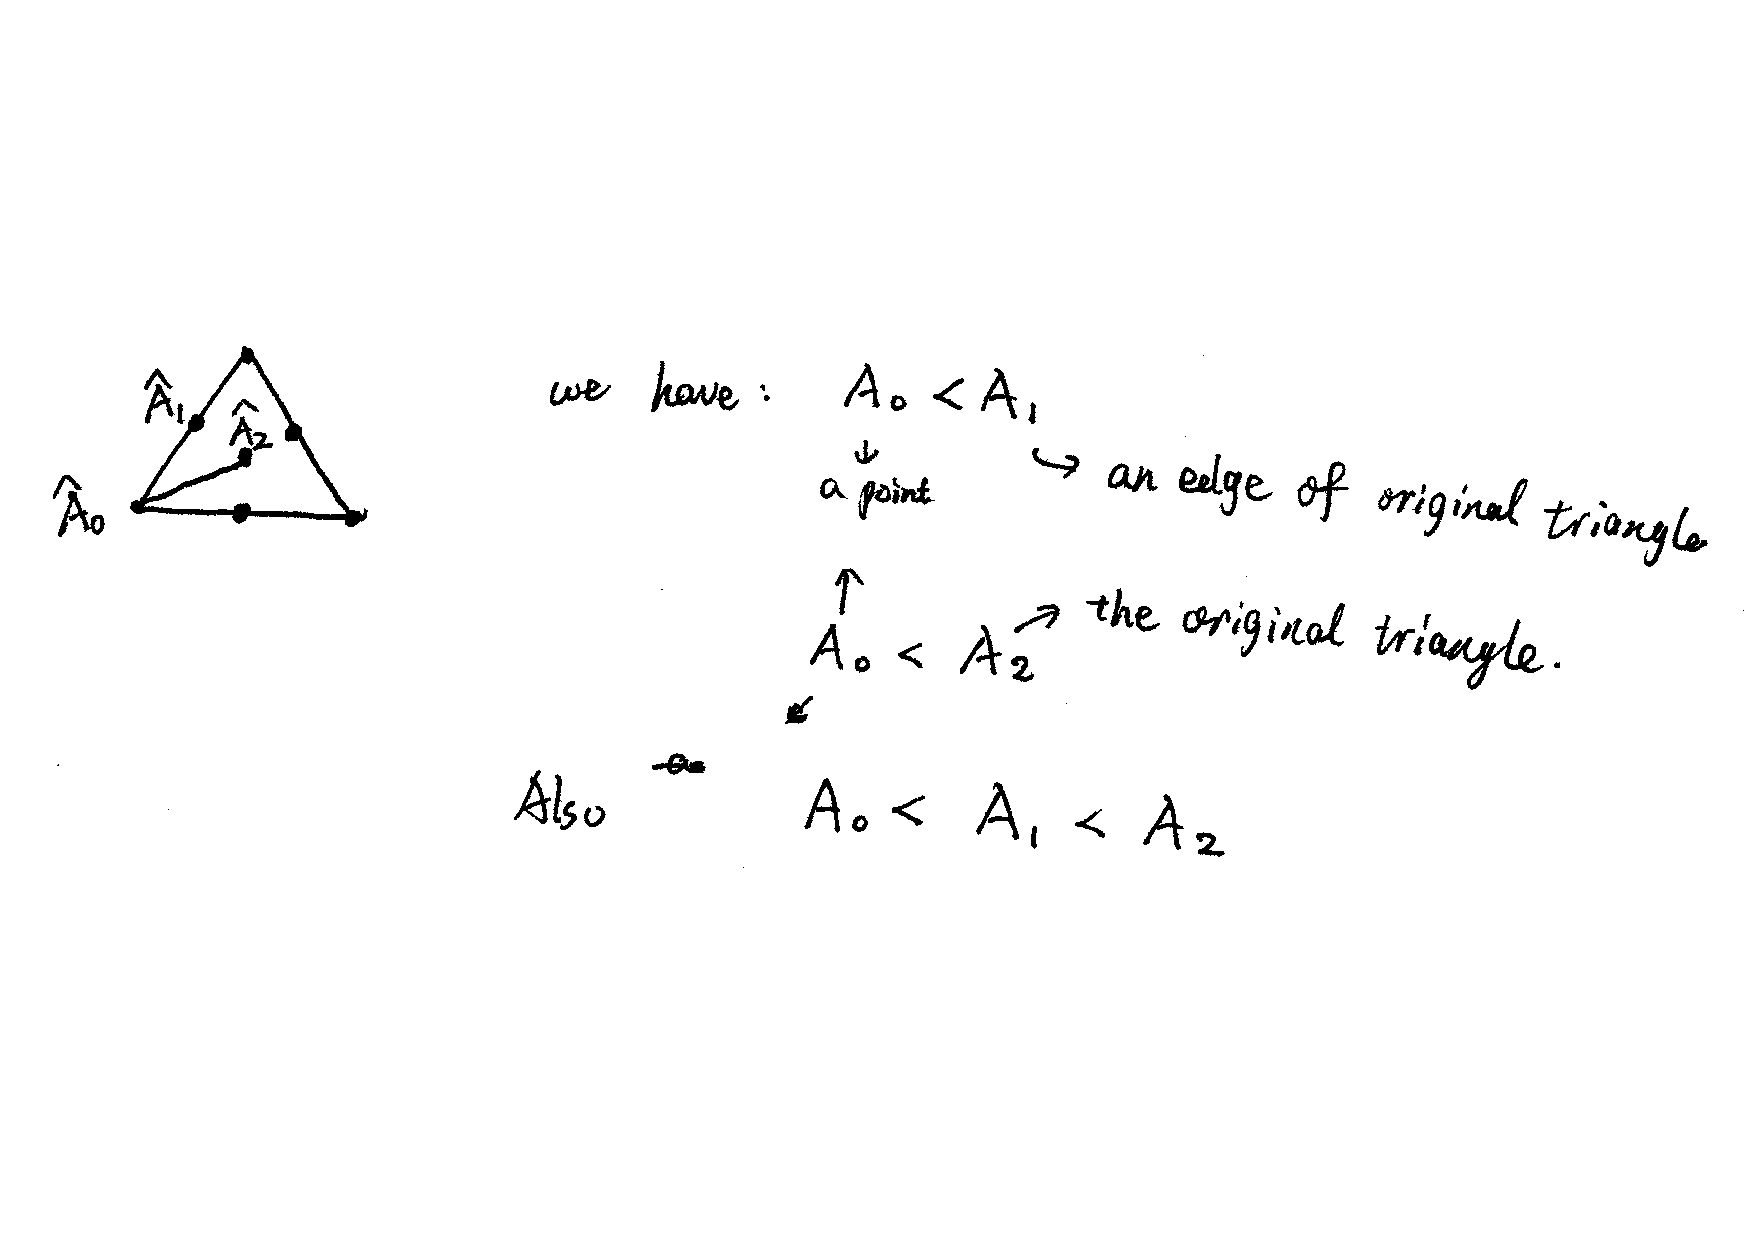
\includegraphics[width=0.9\linewidth]{pics/ch6-scanned-notes-1/p9.pdf}
    \end{figure}
\end{remark}

Now we give a precise description of how this Bary center division
will work. We first describe precisely two characteristics of a
simplicial complex. 

\begin{defi}[dimension of a simplicial complex]
\nomenclature{dimension of a simplicial complex}{\nomrefpage.}
    The dimension of a simplicial complex $K$ is the maximum of the
    dimensions of all its simplexes.
\end{defi}
\begin{defi}[mesh $\mu(K)$]
\nomenclature{mesh $\mu(K)$}{\nomrefpage.}
    The mesh of a simplicial complex $K$ is the maximum of the
    diameters of all its simplexes.
\end{defi}

As we expected, the mesh (which carries the intuition of the smallness
of one simplicial complex) of a simplicial complex will decrease. The
following lemma confirmed this.

\begin{lemma}
    The sollection of simplexes described above forms a simplicial
    complex. If it is denoted by $K^1$, and is called the first
    barycentric subdivision of $K$, then $K^1$ has the following
    properties:
    \begin{enumerate}
        \item each simplex of $K^1$ is contained in a simplex of $K$;
        \item Their topology are the same: $|K^1|=|K|$
        \item If the dimension of $K$ is $n$, then
            \begin{equation}
                \mu(K^1)\leq \frac{n}{n+1}\mu(K)
            \end{equation}
    \end{enumerate}
\end{lemma}
\begin{proof}
    The proof can be found in page 126 to 127 of \cite{book}. But the
    proof of the last point is not so clear and is illustrated here:
\begin{figure}[H]
    \centering
    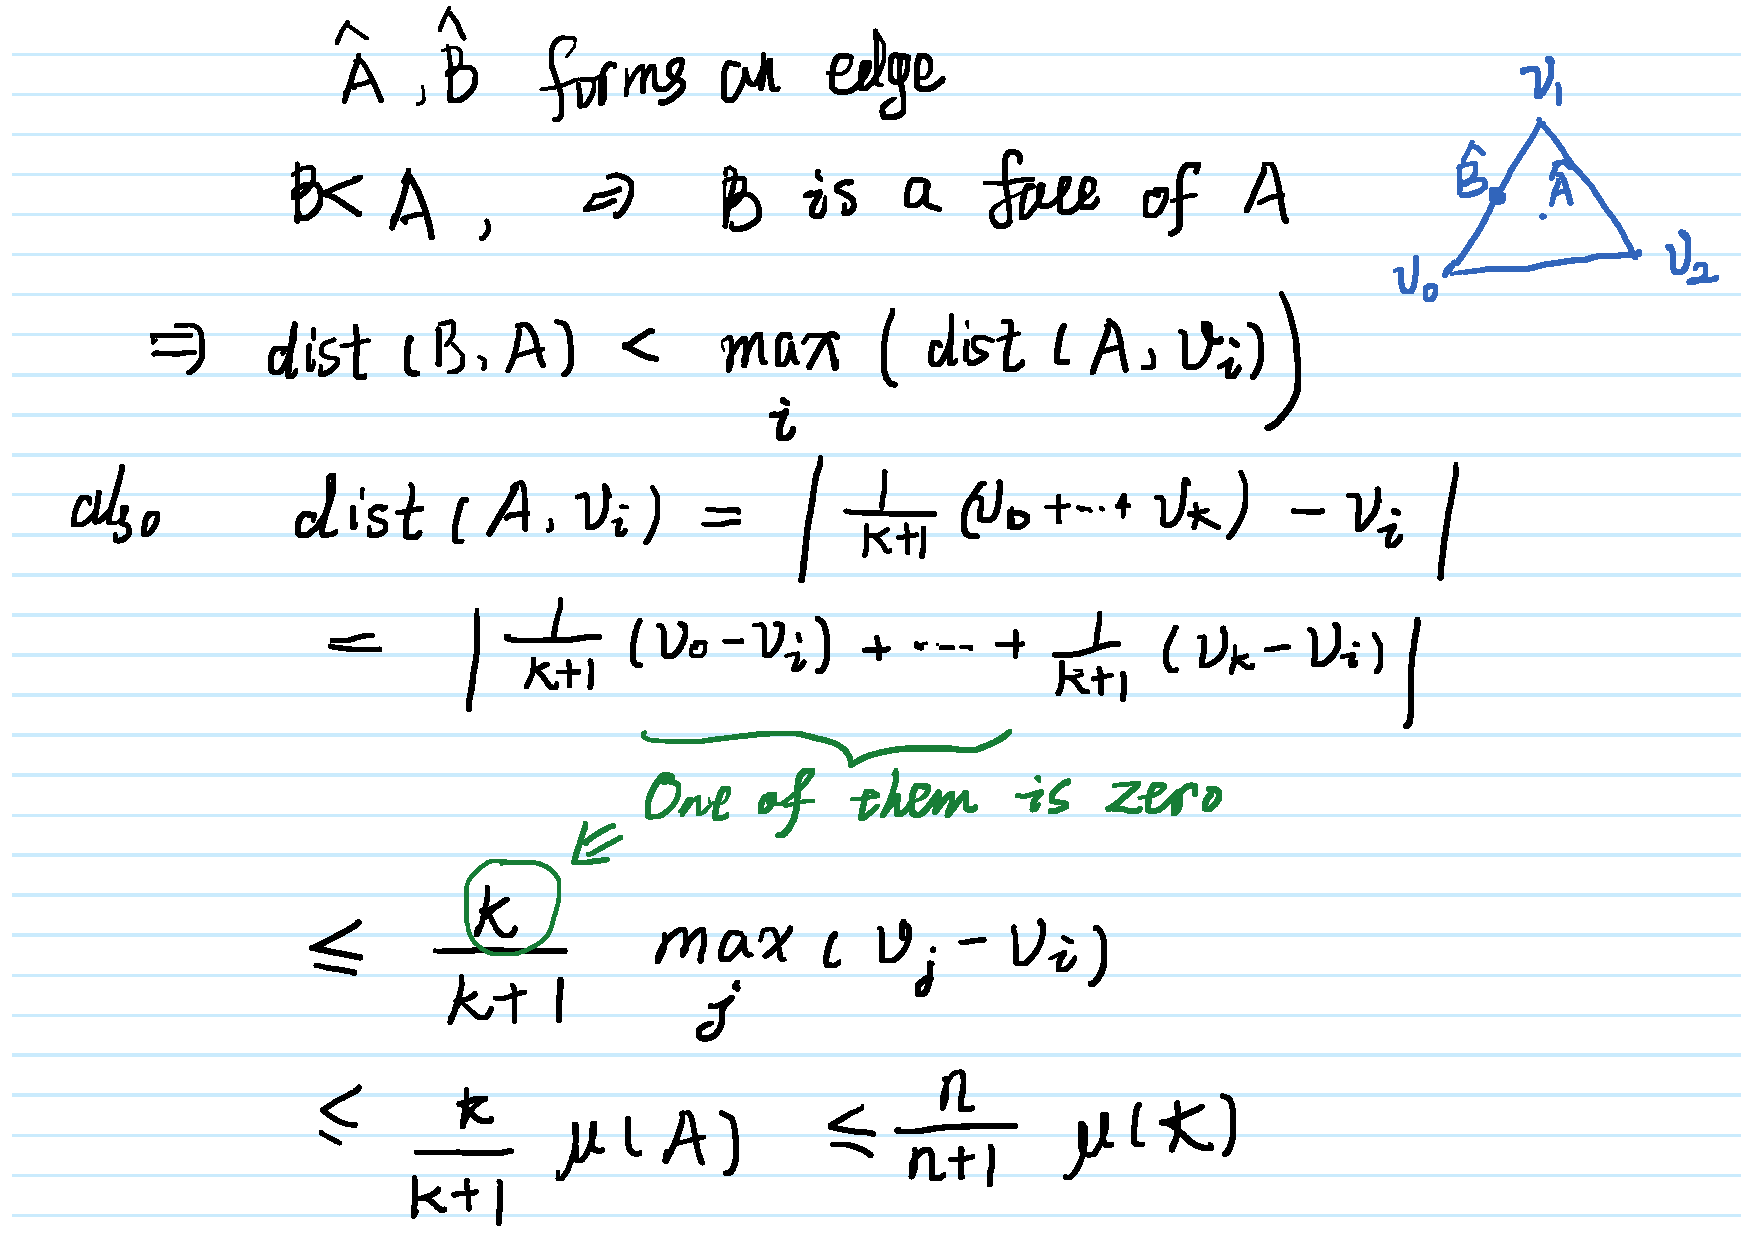
\includegraphics[width=1\linewidth]{pics/ch6-notes-2/explain1.pdf}
\end{figure}
\end{proof}
\begin{remark}
    Notice that the number $\frac{n}{n+1}<1$, hence after an infinite
    number of Barycentric subdivision, the mesh (averaged diameter) of
    a simplicial complex $K^m$ will goes to zero!
\end{remark}
\subsection{Section 6.3 Simplicial approximation}
\label{sec:Simplicial-approximation}

The purpose here is to approximate any continuous map $f:A\to B$ with
linear map, in a way that is compatible with the triangulations on
both $A$ and $B$.
\begin{figure}[H]
    \centering
    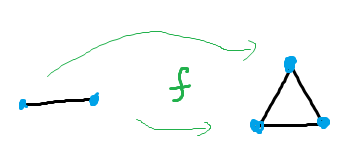
\includegraphics[width=0.4\linewidth]{pics/ch6-notes-2/exp2.png}
\end{figure}
\begin{defi}[Simplicial map]
\nomenclature{Simplicial map}{\nomrefpage.}
    Let $K$ and $L$ be simplicial complexes. A continuous map $s:K\to
    L$ is called simplicial, if it takes simplexes of $K$
    \textit{linearly} to simplexes of $L$. Specifically, being
    \textit{linear} means that:
    
    For $\forall A\in K$, we have $B=s(A)\in L$. Also, if
    $A=\{v_0,\cdots,v_k\}$, then $B=\{s(v_0),\cdots,s(v_k)\}$.
    Lastly, if $x=\sum_{i=0}^k \lambda_i v_i$ is a a point in $A$, with
    $\lambda_i\geq 0$ and $\sum_{i=0}^k\lambda_i=1$, then
    $$s(x) = \sum_{i=0}^k \lambda_i s(v_i)$$

    In a word, $s$ maps simplexes to simplexes, vertices, to vertices,
    and points linearly to points.
\end{defi}
\begin{remark}
    It is easy to see that the a simplicial map is uniquely determined
    by its value on all the vertices. By this, there can only be a
    finite number of such kind of maps, since there are only a finite
    number of vertices.
\end{remark}

Now we want to find such linear maps to approximate a give function
$f:|K|\to |L|$. Given a point $x\in |K|$, we define the
\nomen{carrier of $f(x)$} to be the unique simplex of $L$ that contain
$f(x)$ as its interior point.

\begin{defi}[Simplicial Approximation]
\nomenclature{Simplicial Approximation}{\nomrefpage.}
    A simplicial map $s:|K|\to |L|$ is called a simplicial approximation of
    $f:|K|\to |L|$ if and only if $s(x)\in$ carrier of $f(x)$,
    $\forall x\in |K|$.
\end{defi}
\begin{ex}
    Trivial examples:
\begin{figure}[H]
    \centering
    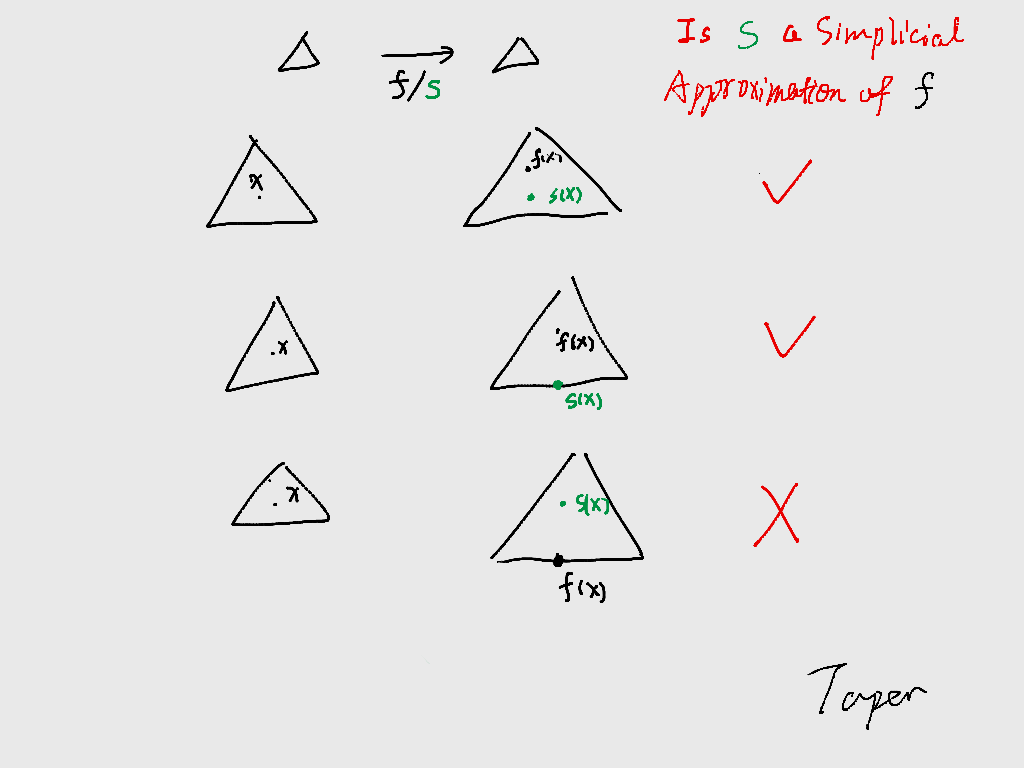
\includegraphics[width=0.8\linewidth]{pics/ch6-notes-2/ex3.png}
\end{figure}
\end{ex}
\begin{ex}
    Now we show that when simplicial approximation does not exits. The
    set up is as follows:
    \begin{figure}[H]
        \centering
        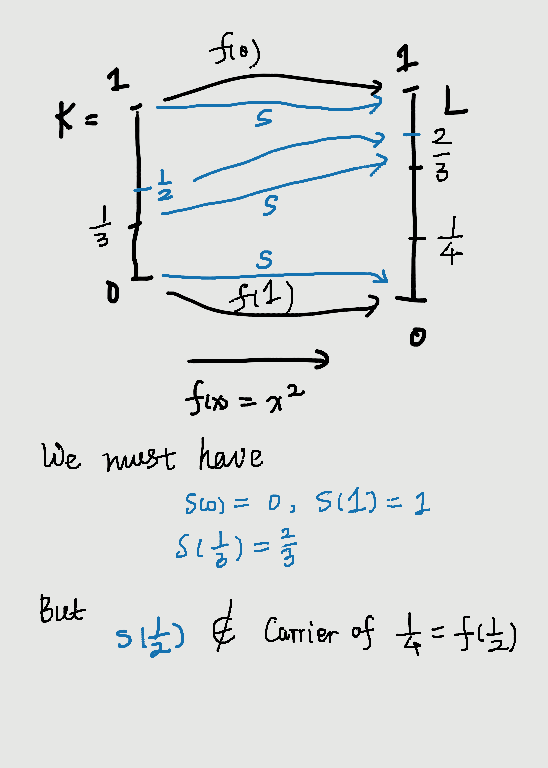
\includegraphics[width=0.8\linewidth]{pics/ch6-notes-2/ex4.png}
    \end{figure}
    Hence, there is no simplicial approximation of $f$. But, it will
    be shown below that, if we divide $K$ small enough
    ($K^1,K^2,\cdots$), we will eventually be able to find a
    simplicial approximation of $f$ in some $K^n$.
\end{ex}

\begin{thm}[Simplicial approximation theorem]
    \label{thm:SAT}
    Let $f:|K|\to |L|$ be a continuous map between polyhedras formed
    by simplicial complexes $|K|$ and $|L|$. If $m$ is chosen large
    enough, then there is a simplicial approximation $s:|K^m|\to|L|$
    to $f:|K^m|\to|L|$.
\end{thm}
The proof will use a lemma. Define the \nomen{open star} $v$ of a
simplicial complex $K$, as the union of the interiors of those
simplexes of $K$ having $v$ as a vertex. This union is denoted by
\nomen{$\operatorname{star}(v,K)$}. An example is:
\begin{figure}[H]
    \centering
    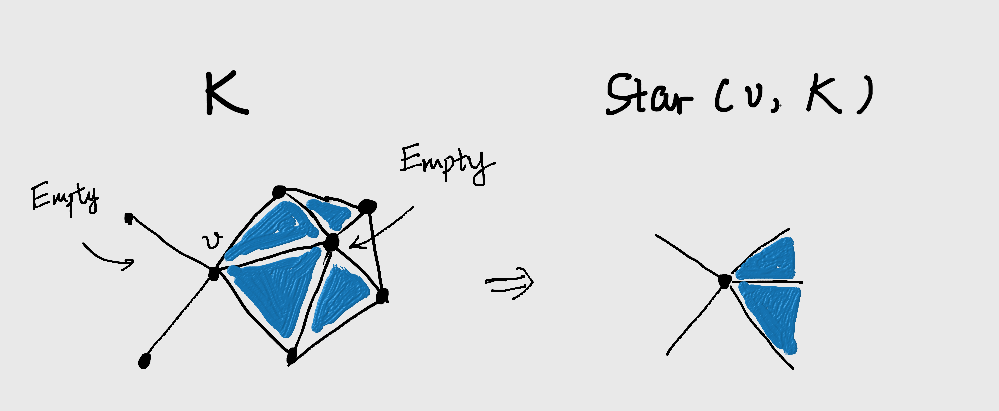
\includegraphics[width=1.0\linewidth]{pics/ch6-notes-2/ex5.png}
    \caption{Example of star}
\end{figure}
So it really feels like a star spreading out from $v$. We have

\begin{lemma}
    Vertices $v_0,v_1,\cdots,v_k$ of a simplicial complex $K$ are the
    vertices of a simplex of $K$ if and only if the intersection of
    their open stars is nonempty, i.e. 
    $$\cup_0^k \operatorname{star}(v_i,K)\neq\emptyset$$
\end{lemma}
\begin{proof}
    The proof can be found in page 130 of \cite{book}. It is quite
    trivial.
\end{proof}
Then we have the \textbf{proof of theorem \ref{thm:SAT}}:
\begin{proof}
    The proof is found in page 130 to 131 of \cite{book}. The idea is
    that if for each vertex $u$ of $K$, we can find a vertex $v$ of
    $L$ such that
    \begin{equation}
        f(\operatorname{star}(u,K))\subseteq\operatorname{star}(v,L)
        \label{eq:proof-temp} \tag{*} 
    \end{equation}
    Then the simplicial map $s(u)=v$ will be easily verified to be a
    simplicial approximation of $f$. 
    
    To make such (*) happen, we naturally have to divide $K^m$ small
    enough. We can achieve such small division is guaranteed by the
    Lebesgue lemma \ref{lemma:lebesgue-lemma}, since each subdivision
    makes the averaged diameter smaller.
\end{proof}

\subsection{Section 6.4 The edge group of a complex}
\label{sec:edge-group}

The definition of edge group is so similar to that of fundamental
group (actually, edge group is made to simplify computation of
fundamental group). Therefore, I will not waste too much words here.
One with reasonable intuition could just skim through this section.

The following excerpt from book \cite{book} best captures the idea:

\begin{myquote} \enquote{
We calculated the fundamental groups of one or two spaces in Chapter
5, but our calculations, though efficient for the examples given
there, were rather \textit{ad hoc}. If we agree to work with triangulable
spaces, we can be much more systematic. We shall show how to read off
generators and relationst for the fundamental group from a
triangulation of the space.

Let $X$ be a path-connected triangulable space, take a specific
triangulation $h:|K|\to X$, and replace $X$ by $|K|$ (we are at
liberty to do this since the funda- mental group is a topological
invariant). Now the advantage of a polyhedron $|K|$ is that the
elements of its fundamental group can be represented by loops which
are made up of edges of $K$. Using such 'edge loops' we shall
construct a group, called the edge group of the complex $|K|$, which
can be computed and wh ich is isomorphic to the fundamental group of
$|K|$.
} \end{myquote}

The edge pathes $v_0,v_1,\cdots,v_k$, edge loops
$v,v_1,\cdots,v_{k-1},v$ are defined similar to pathes and loops.
The equivalence relation between edge loops are defined as represented
by the following drawing:
\begin{figure}[H]
    \centering
    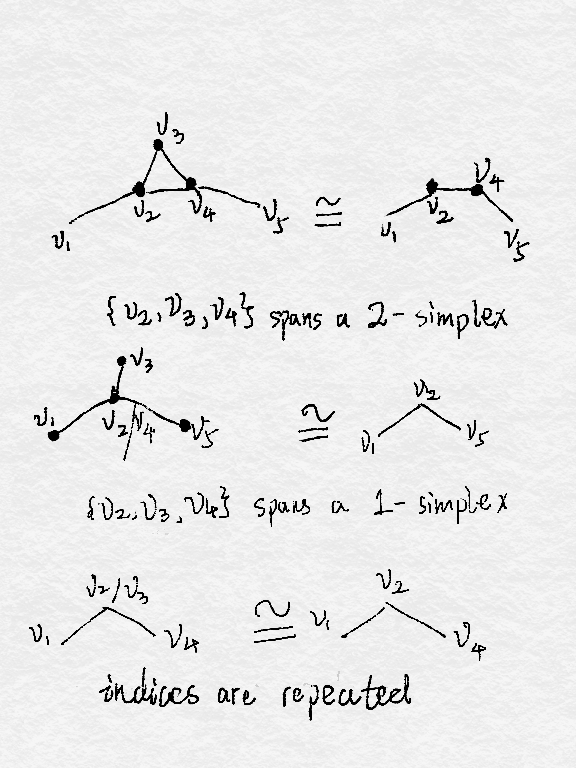
\includegraphics[width=0.8\linewidth]{pics/ch6-notes-2/edge-group1.png}
\end{figure}

The equivalence class of edge pathes and edge loops are denoted
$\{v_0,v_1,\cdots,v_k\}$, and $\{v,v_1,\cdots,v_{k-1},v\}$,
respectively. The multiplication of edge loops is defined simply as
\begin{equation}
    \{v,v_1,\cdots,v\}\{v,w_1,\cdots,v\} =
    \{v,v_1,\cdots,v,w_1,\cdots,v\}
\end{equation}

It is trivially verified that such edge loops form a group, called the
\nomen{edge group based at $v$, $E(K,v)$}. It is also trivially
verified that such group does not depend on the choice of base point
$v$, since $|K|$ is path-connected.

\begin{thm}
    $E(K,v)$ is isomorphic to $\pi_1(|K|,v)$
\end{thm}
\begin{proof}
    The proof can be found on page 133 of \cite{book}. The essential
    idea is that an edge loop is just a loop. And a loop is just a
    continuous map $f:I\to |K|$, we can easily use the simplicial
    approximation $s:I^m\to |K|$ of $f$ (with appropriately $m$), to
    find a corresponding edge loop.

    The uniqueness of the loop corresponding to an edge loop is found
    again by treating $L:=I^2$ as a simplicial complex and apprximate
    again the homotopy $F:L\to |K|$. The resulted $S$ will again gives
    us a equivalence relation to the constant edge loop. (Note, we
    have to use the fact the simplicial maps preserves the equivalence
    relation between edge pathes). The following pictorially
    produces the proof:
    \begin{figure}[H]
        \centering
        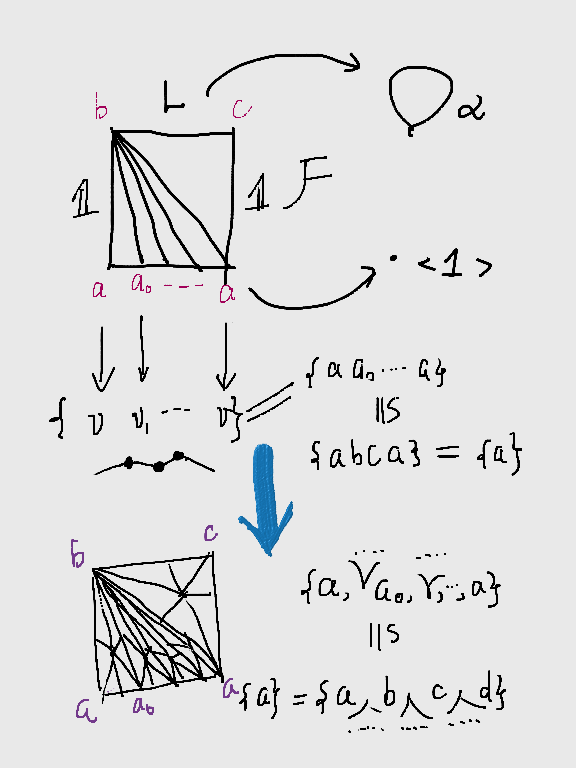
\includegraphics[width=0.9\linewidth]{pics/ch6-notes-2/L.png}
    \end{figure}
\end{proof}

\begin{remark}
    This theorem already tells us that the Edge group $E(K,v)$ is
    indepedent on the choice of base point $v$, since our polyhedron
    $|K|$ is always assumed to be path-connected.
\end{remark}

Based on this edge group, we will try to calculate more explicitly the
structure of this group. Here we provide a way to get the generators
and relations directly from the edge group.

\begin{key}
    The intuition is that the structure of this group is
    determined only by those $1$-simplexes, $2$-simplexes, and the
    equivalence relations between edge pathes. All higher dimensional
    simplexes are not relevent to this group structure.
\end{key}

We let \nomen{$L$} the subcomplex of a simplicial complex $K$. This
subcomplex $L$ is required to contain all the vertices of $K$ and such
that its polyhedron $|L|$ is path-connected and simply-connected. Can
we find such a subcomplex? The intuitive answer is yes due to the
path-connectedness nature of $|K|$. The rigorous answer needs the help
of a concept \nomen{tree}. A tree $T$ is a one-dimensional subcomplex of
$K$ whose polyhedron $|T|$ is both path-connected and
simply-connected. The following lemma affirms that we can find our $L$
to be exactly the maximal tree in $K$:
\begin{lemma}
    A maximal tree contains all the vertices of $K$.
\end{lemma}
\begin{proof}
    We first observe that a tree must exists, unless the dimension of
    $K$ is $0$ (in which case, there is entirely no need for the
    following discussions, and the lemma is still true because there is
    not even a maximal tree!). Let $T$ be a maximal tree in $K$, which
    means that if $T'$ is a tree and contains $T$, than $T'=T$. 
    The next step is simply and is expatiated on page 134 of
    \cite{book}. The idea is to grow a tree by adding more vertices,
    which is possible because $|K|$ is path-connected and a path can
    be easily turned into an edge path. Note that add a
    simply-connected space in this way will keep the space
    simply-connected, just do not add a vertices twice too creat a
    loop. 
    
    Obviously one will get a tree which is maximal and contains all
    the vertices.  Such a process also affirms that the maximal tree
    will exist (but may not be unique).
\end{proof}

\begin{ex}
    Here is the maximal tree of a triangulation:
    \begin{figure}[H]
        \centering
        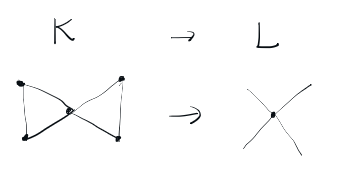
\includegraphics[width=0.6\linewidth]{pics/ch6-notes-3/ex1-maximal-tree.png}
    \end{figure}
\end{ex}

\begin{ex}
    The maximal tree is usually not unique!
    \begin{figure}[H]
        \centering
        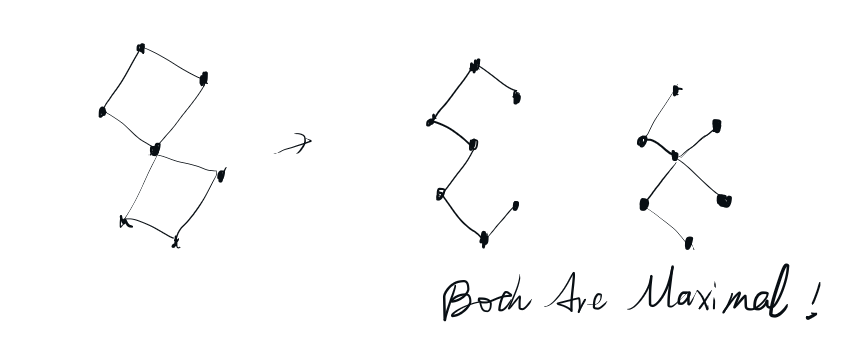
\includegraphics[width=0.9\linewidth]{pics/ch6-notes-3/ex2-maxi-tree-not-unique.png}
    \end{figure}
\end{ex}


Now since $|L|$ is simply-connected, it will not contribute to the
edge group. What contributes to the edge group is those edges that are
not in this $|L|$. This motivates us to define a new group:

\begin{defi}[$G(K,L)$]
\nomenclature{$G(K,L)$}{\nomrefpage.}
    Let $L$ be the maximal tree in $K$ (assume $|K|$ is
    path-connected). Then $G(K,L)$ is defined by generators $g_{ij}$
    for each \textbf{ordered} pair of vertices $v_i,v_j$ such that
    $\{v_i,v_j\}$ spans a simplex ($0$-simplex or $1$-simplex) in $K$.
    Those generators are subject to the following conditions:
    \begin{enumerate}
        \item $g_{ij}=1$, the identity element, if and only if
            $\{v_i,v_j\}$ spans a simplex in $L$.
        \item $g_{ij}g_{jk}=g_{ik}$ if and only if $\{v_i,v_j,v_k\}$
            spans a simplex ($0$ or $1$ or $2$ simplex) in $K$.
    \end{enumerate}
\end{defi}

\begin{ex}
    \label{ex:torus-GLKgroup}
    Again, for circle:
    \begin{figure}[H]
        \centering
        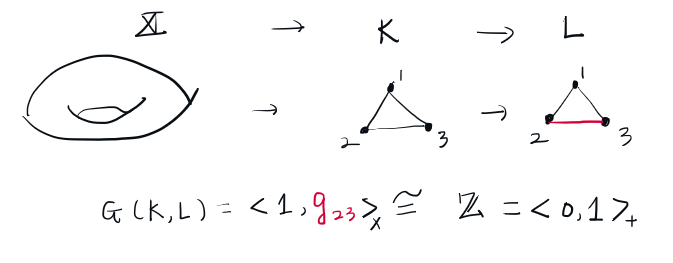
\includegraphics[width=0.9\linewidth]{pics/ch6-notes-3/ex3-L-in-triangle.png}
    \end{figure}
\end{ex}
\begin{ex}
    \label{ex:ex4-L-in-two-torus}
    And for another:
    \begin{figure}[H]
        \centering
        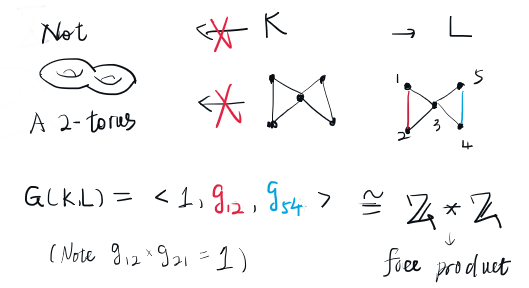
\includegraphics[width=0.9\linewidth]{pics/ch6-notes-3/ex4-L-in-two-torus.png}
    \end{figure}
    Note that this does not gives a triangulation of two-torus! 
    The reason will be explained later in
    example~\ref{ex:pi1-two-torus}.
\end{ex}
More generally, we have
\begin{thm}
    $G(K,L)\cong E(K,v)$, as a group isomorphism.
\end{thm}
\begin{proof}
    The proof in page 135 to 136 of \cite{book} constructs the
    following homomorphisms:

    $$\begin{tikzcd}[]
        G(K,L)\ar[r,"\phi",shift left] & 
            E(K,v)\ar[l,"\theta", shift left]
    \end{tikzcd}$$

    It is pretty simple to get these two maps and confirms that their
    composites are identity functions on each space.
\end{proof}

\begin{remark}
    We have now the following chain of homomorphisms:
    $$ \pi_1(|K|,v)\cong E(K,v) \cong G(K,L) $$
\end{remark}
\begin{coro}
    For any path-connected, triangulable space, its fundamental group
    is finitely presented, i.e., the fundamental group has only a
    finite number of generators and a finite number of relations.
\end{coro}

For example, we have demonstrated in example~\ref{ex:torus-GLKgroup}
that its $G(K,L)\cong \Z_2$, which is just its fundamental group.

In addition, armed with this tool, we can answer an additional
question. We want to know what is the fundamental group of two torus
connected together:

\begin{figure}[H]
    \centering
    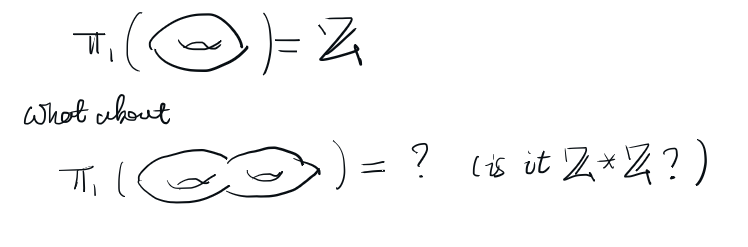
\includegraphics[width=0.9\linewidth]{pics/ch6-notes-3/pic-two-torus.png}
\end{figure}

This can be done using the following theorem:

\begin{thm}[Van Kampen's theorem]
    Let $J$, $K$ be two simplicial complexes in some Euclidean space
    which intersect in a common subcomplex, and suppose all $|J|$,
    $|K|$, $|J\cap K|$ are path-connected. Let $j,k$ be the inclusion
    maps:
    $$ \begin{tikzcd}[]
        \lvert J\cap K\rvert \ar[r,"j",hook] & \lvert J\rvert
    \end{tikzcd}$$
    $$ \begin{tikzcd}[]
        \lvert J\cap K\rvert \ar[r,"k",hook] & \lvert K\rvert
    \end{tikzcd}$$
    Take a vertice $v\in J\cap K$ as the base point. The fundamental
    group $\pi_1(|J\cup K|, v)$ is obtained from the free product
    $\pi_1(|J|,v)*\pi_1(|K|,v)$ by adding the relations
    $j_*(z)=k_*(z)$ for all $z\in\pi_1(|J\cap K|,v)$.
\end{thm}
\begin{proof}
    The proof can be found on page 137 to 138 of \cite{book}. Please
    do read the paragraph just before this theorem to get a picture of
    the proof.

    Note also that a $2$-simplex cannot possiblly cross the
    intersection part $J\cap K$. Please check why I mention this when
    reading the proof on the book \cite{book}.
\end{proof}

\begin{ex}
    \label{ex:pi1-two-torus}
    Here's how to find the fundamental group for two-torus connected:
\begin{figure}[H]
    \centering
    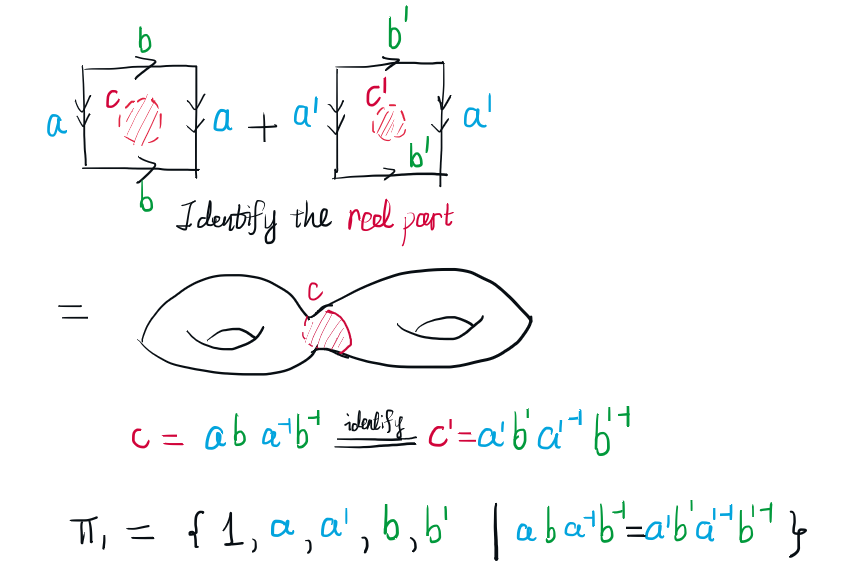
\includegraphics[width=0.9\linewidth]{pics/ch6-notes-3/ex-pi1-two-torus.png}
\end{figure}
    The result confirms that the triangulation of a two-torus is as
    simple as in example~\ref{ex:ex4-L-in-two-torus}.
\end{ex}

\begin{ex}
    Next we consider the projective space $\R P^2$, the space is
    homeomorphic to half the sphere $S^2$, with the antipodal points
    on the boundary identified:
    \begin{figure}[H]
        \centering
        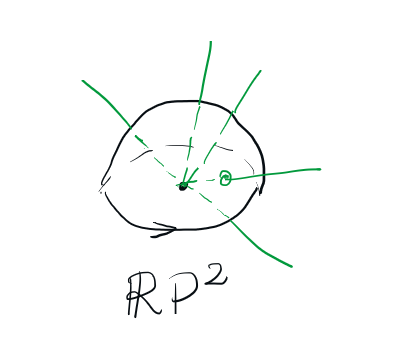
\includegraphics[width=0.4\linewidth]{pics/ch6-notes-3/rp2.png}
    \end{figure}
    Then it can be regarded as a 2-disc with it boundary attached to
    the boundary of a M\"obius strip. This construction will tell us
    that the fundamental group of $\R P^2$ is $\Z_2$.
    \begin{figure}[H]
        \centering
        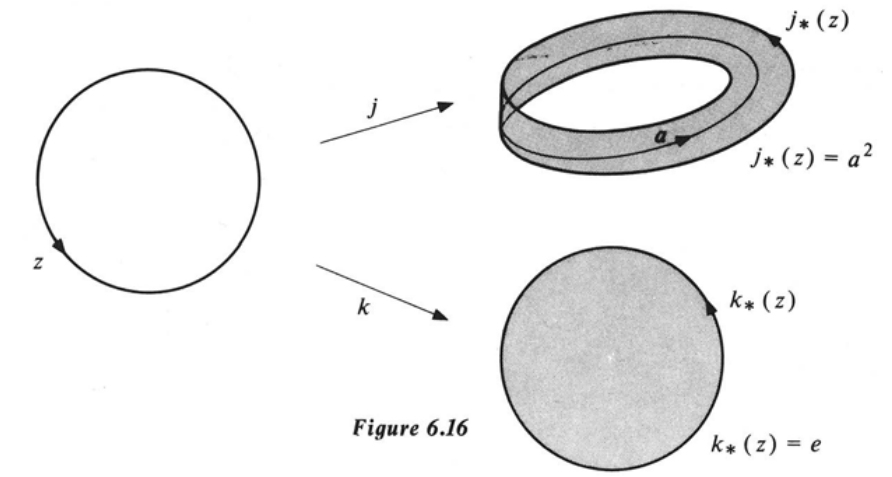
\includegraphics[width=0.8\linewidth]{pics/ch6-notes-3/rp2-pi1.png}
        \caption{Page 139, Fig 6.16 of \cite{book}}
    \end{figure}
\end{ex}

